\section{Ejemplos}\label{Examples}

\setbeamercolor{block title}{bg=blue!50!black,fg=white}
\setbeamercolor{block body}{bg=blue!20,fg=white}

\begin{frame}
    \begin{columns}[t]
        \begin{column}{.5\textwidth}
          \tableofcontents[sections={1-2},currentsection]
        \end{column}
        \begin{column}{.5\textwidth}
          \tableofcontents[sections={3-4},currentsection]
        \end{column}
    \end{columns}
\end{frame}

\subsection{TF-IDF}

\begin{frame}[fragile]{TF-IDF}

\only<1-4>{\begin{center}
    \begin{block}{Teniendo las siguientes oraciones:}
        \begin{itemize}
            \item[-]<1-4>{El río Danubio pasa por Viena, su color es azul.}
            \item[-]<2-4>{El caudal de un río asciende en Invierno.} 
            \item[-]<3-4>{El río Rhin y el río Danubio tienen mucho caudal.} 
            \item[-]<4>{Si un río es navegable, es porque tiene mucho caudal.}    
        \end{itemize}
    \end{block}
\end{center}}

\pause 

    \only<4>{A continuación, obviando las palabras más comunes(que normalmente son eliminadas en este mismo proceso),
    será mostrado el proceso al que es sometida toda la información usando las fórmulas ya presentadas.}

    \only<5>{\begin{figure}[h]
        \center
        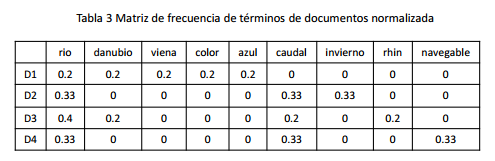
\includegraphics[width=6cm]{ejtf.jpg}
        \caption{Calculando el TF}
    \end{figure}}

    \only<6>{\begin{figure}[h]
        \center
        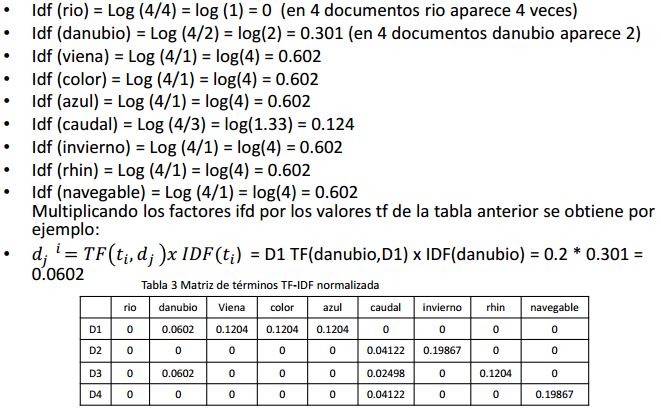
\includegraphics[width=6cm]{ejidf.jpg}
        \caption{Obteniendo la matriz TF-IDF}
    \end{figure}}

    \only<7>{\begin{figure}[h]
        \center
        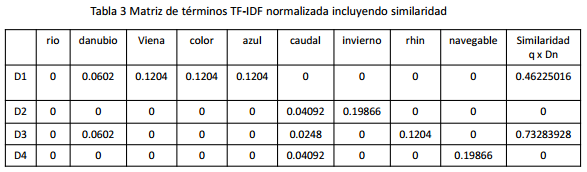
\includegraphics[width=6cm]{ejcos.jpg}
        \caption{Calculando la Similitud de cosenos}
    \end{figure}}
    
\end{frame}

